%\documentclass{article}
%\usepackage{graphicx,psfrag,epsfig,epsf,latexsym,hhline,amsmath,amssymb,multirow}
%\usepackage[usenames,dvipsnames]{pstricks}
%\usepackage{pst-plot}
%\usepackage{pstricks-add}
%\usepackage{color}
%\usepackage{stmaryrd}
%\usepackage{makecell}
%
%\interdisplaylinepenalty=2500
%\usepackage{graphicx}
%\usepackage{amsthm}
%\usepackage{footnote}
%
%\usepackage{blindtext}
%\usepackage{etoolbox}
%
%\usepackage{tikz}
%\usepackage{pgfplots}
%\usepgflibrary{shapes}
%\usetikzlibrary{arrows,shapes,chains,matrix,positioning,scopes,patterns	}
%\pgfplotsset{compat=newest}
%\pgfplotsset{plot coordinates/math parser=false}
%
%\begin{document}
%\centering
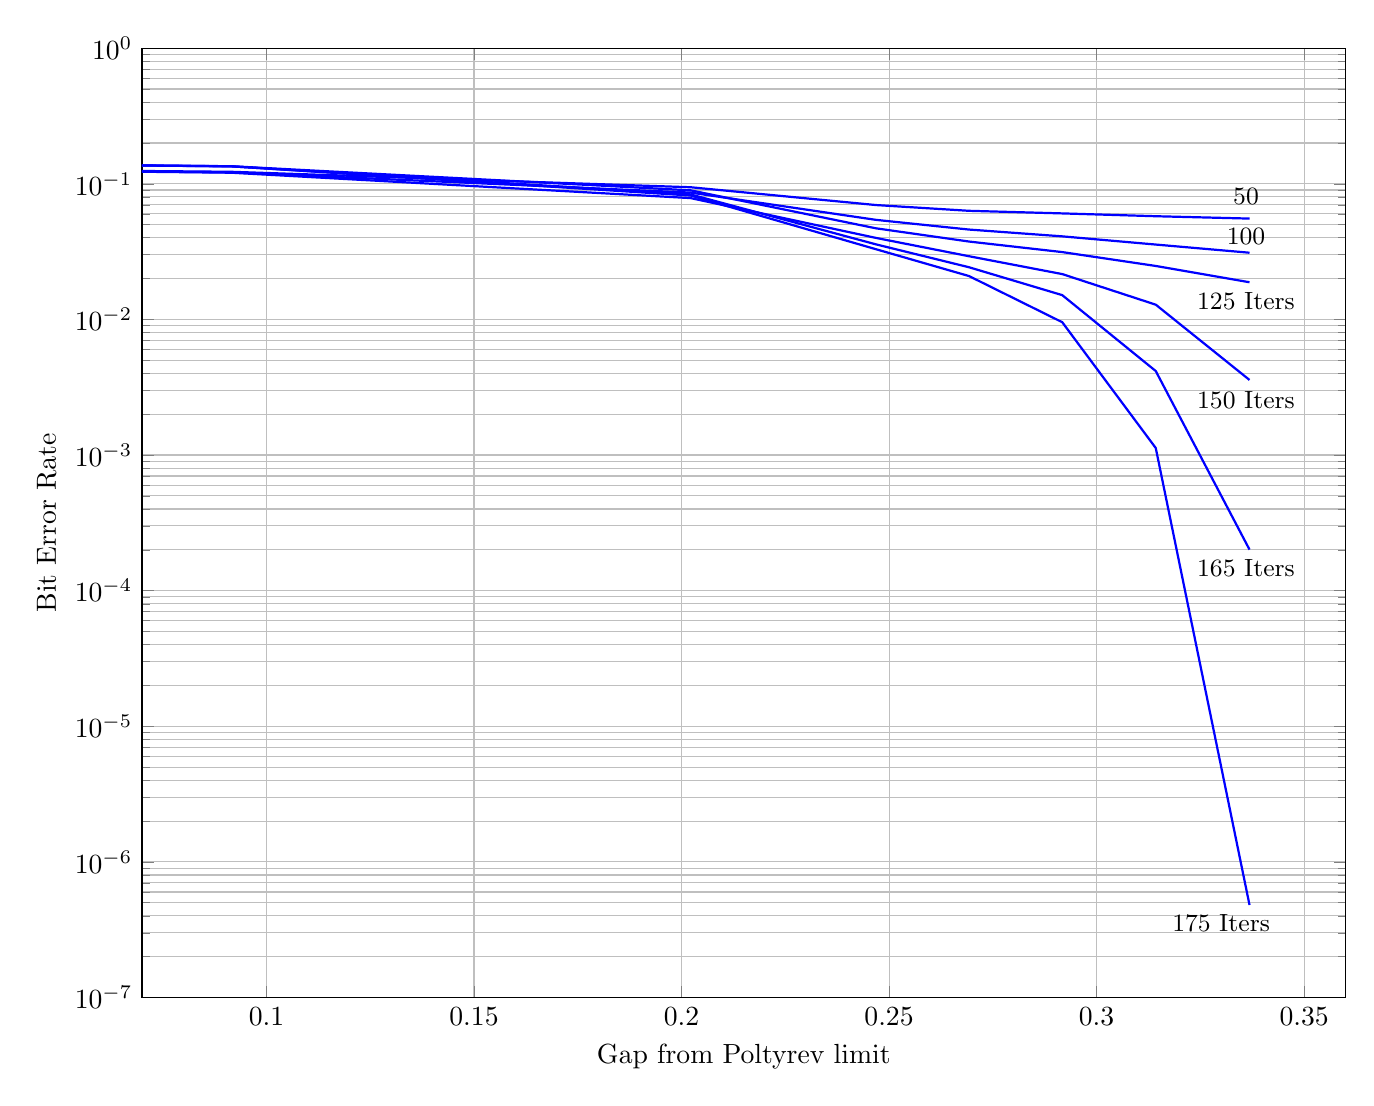
\begin{tikzpicture}
\centering
\begin{axis}[
width=6.01828521434821in,
height=4.74667979002625in,
scale only axis,
xmajorgrids,
ymajorgrids,
yminorgrids,
xmin=0.07,
xmax=0.36,
ymode=log,
ymin=1e-07,
ymax=1,
yminorticks=true,
xtick = {0,0.05,...,0.36}, % make steps of length 0.4
xlabel={Gap from Poltyrev limit},
ylabel={Bit Error Rate}
]
\addplot [color=blue,solid,forget plot,thick]
  table[row sep=crcr]{-0.0177322806931892	0.131282232945261\\
0.0915256333368557	0.122591784109477\\
0.202175405336076	0.0942922155841503\\
0.246833033981915	0.0697083460988562\\
0.269248245487832	0.0632015165441177\\
0.291721452430959	0.0604816687091503\\
0.314252955696046	0.0576518203635621\\
0.336843058515443	0.0553889144199346\\
};
\node[font=\small, above] at (axis cs:0.336,0.06){50 };

\addplot [color=blue,solid,forget plot,thick]
  table[row sep=crcr]{-0.0177322806931892	0.131267552593954\\
0.0915256333368557	0.121379378574346\\
0.202175405336076	0.0861130259395425\\
0.246833033981915	0.054207337622549\\
0.269248245487832	0.0459767029207516\\
0.291721452430959	0.040962992749183\\
0.314252955696046	0.0356387229370915\\
0.336843058515443	0.031020012084695\\
};
\node[font=\small, above] at (axis cs:0.336,0.03){100 };

\addplot [color=blue,solid,forget plot,thick]
  table[row sep=crcr]{-0.0177322806931892	0.144683478860294\\
0.0915256333368557	0.134713286356209\\
0.202175405336076	0.0894630182802288\\
0.246833033981915	0.0469594822303922\\
0.269248245487832	0.0375147569444444\\
0.291721452430959	0.0313596686070261\\
0.314252955696046	0.0247765522875817\\
0.336843058515443	0.0187923219635076\\
};
\node[font=\small,below] at (axis cs:0.336,0.0187){125 Iters};

\addplot [color=blue,solid,forget plot,thick]
  table[row sep=crcr]{-0.0177322806931892	0.131289253982843\\
0.0915256333368557	0.120674721711601\\
0.202175405336076	0.0784403084150327\\
0.246833033981915	0.0398978502859477\\
0.269248245487832	0.029233660130719\\
0.291721452430959	0.021585631127451\\
0.314252955696046	0.0128414649714052\\
0.336843058515443	0.00357706120642702\\
};
\node[font=\small,below] at (axis cs:0.336,0.0035){150 Iters};

\addplot [color=blue,solid,forget plot,thick]
  table[row sep=crcr]{-0.0177322806931892	0.14470805249183\\
0.0915256333368557	0.134422551572712\\
0.202175405336076	0.0834944980596405\\
0.246833033981915	0.0357638378267974\\
0.269248245487832	0.024248148999183\\
0.291721452430959	0.0151024050245098\\
0.314252955696046	0.00416107536764706\\
0.336843058515443	0.000200708061002179\\
};
\node[font=\small,below] at (axis cs:0.336,0.000201){165 Iters};

\addplot [color=blue,solid,forget plot,thick]
  table[row sep=crcr]{-0.0177322806931892	0.144707095077614\\
0.0915256333368557	0.134512548508987\\
0.202175405336076	0.0819230621936275\\
0.246833033981915	0.0329302108864379\\
0.269248245487832	0.0208807700163399\\
0.291721452430959	0.00953257761437908\\
0.314252955696046	0.00112607230392157\\
0.336843058515443	4.80834694989107e-07\\
};
\node[font=\small,below] at (axis cs:0.33,4.8 e-07){175 Iters};

\coordinate (left_bottom_pt) at ( axis cs:0.1,-0.1);
\coordinate (right_top_pt) at (axis cs:0.4,1);
\useasboundingbox (left_bottom_pt) rectangle ( right_top_pt);
\end{axis}


\end{tikzpicture}
%\end{document}